%%%%%%%%%%%%%%%%%%%%%%%%%%%%%%%%%%%%%%%%%%%%%%%%%%%%%%%%%%%%%%%%%%%%%%%%%%%%%%%
%%%% SIMPLIFIED SETTINGS WITH ONLY THE INPUTS NEEDED FOR THE COVER IMAGE.
%%%%%%%%%%%%%%%%%%%%%%%%%%%%%%%%%%%%%%%%%%%%%%%%%%%%%%%%%%%%%%%%%%%%%%%%%%%%%%%

\usepackage{xifthen}
\usepackage{lipsum} % Lorem Ipsum



\newcommand{\setMinimalMode}
{
    \isMinimal
    {

        \ifthenelse{\equal{\jobname}{\detokenize{portfolio_document}}}
        {
            \includeonly{ %to run individuals fragments
            % elements/portfolio_meta_data/portfolio_meta_data,
            % elements/portfolio_title_page/portfolio_title_page,
            % elements/preface/preface
            }
        }
        {
            \addonlyfiles{
                % substance,
                % glossary,
                % abreviations,
                body
            }
        }

        % \setbool{isDraft}{true} % true or false
        \setbool{isPrintVersion}{false} % true or false
        \setbool{isDrawRibbons}{false} % true or false
        \setbool{isIncludeMeta}{false} % true or false
        \setbool{isIncludeArticleCover}{false} % true or false
        \setbool{isIncludeToC}{false} % true or false
        \setbool{isIncludeLoF}{false} % true or false
        \setbool{isIncludeLoT}{false} % true or false
        \setbool{isIncludeLoTB}{false} % true or false
        \setbool{isIncludeBiblio}{false} % true or false
        \setbool{isIncludeGlossary}{false} % true or false
        \setbool{isIncludeAbreviations}{false} % true or false
        \setbool{isPrintUnusedGlossary}{false} % true or false
        \setbool{isPrintUnusedAbreviations}{false} % true or false
        \setbool{isHighlightGlossaryAndAbreviations}{false}  % true or false
        \setbool{isIncludeMissingBibEntries}{false} % true or false
        \setbool{isIncludeFootnotes}{false} % true or false
        \setbool{isIncludeCitations}{false} % true or false
        \setbool{isIncludeCitationsInFootnotes}{false} % true or false
        \setbool{isIncludeTextBoxes}{false} % true or false
        \setbool{isMoveTextBoxesToEndOfArticle}{false}  % true or false
        \setbool{isConstrainFloats}{false}  % true or false
        \setbool{isIncludeArticleCoverImgInBody}{false}  % true or false
        \setbool{isCreditsInArticleBody}{false}  % true or false
        \setbool{isSplitInTwoColumns}{false} % true or false
        \setbool{isLandscapeMode}{false} % true or false
        \setbool{isIncludeAppendix}{false} % true or false

        %%%% PORTOFOLIO SPECIFIC:
        \setbool{isIncludePerArticleToC}{false} % true or false
        \setbool{isIncludePerArticleLoF}{false} % true or false
        \setbool{isIncludePerArticleLoT}{false} % true or false
        \setbool{isIncludePerArticleSubstance}{false} % true or false
        \setbool{isSplitBibliographyByChapter}{false}  % true or false

        %%%% OTHER SETTINGS:
        \pagecolor{black}% bg color
        \color{white}% text color
    }
    {}
}

\AfterPreamble{
    \setMinimalMode
}

%%% ===== MACRO TO RUN CONTENTS ONLY IN DRAFT VERSION
\newcommand{\isMinimal}[2]{%
    \ifthenelse{\boolean{isMinimal}}%
    {#1}%
    {#2}%
}

% make sure to update language in document as well
% ENGLISH (EN)
\ifthenelse{\equal{\myLanguage}{en}}{
  \usepackage[english]{babel}
  \usepackage[en-GB]{datetime2}
  \newcommand{\myLanguageLong}{english}
  %
  %
  %
  \newcommand{\TEXTcover}{Cover}
  \newcommand{\TEXTtoc}{Table of Contents}
  \newcommand{\TEXTlof}{List of Figures}
  \newcommand{\TEXTlot}{List of Tables}
  \newcommand{\TEXTpToc}{Partial Table of Contents}
  \newcommand{\TEXTpLof}{Partial List of Figures}
  \newcommand{\TEXTpLot}{Partial List of Tables}
  \newcommand{\TEXTlotb}{List of Textboxes}
  \newcommand{\TEXTmainSource}{Main source}
  \newcommand{\TEXTtextbox}{Textbox}
  \newcommand{\TEXTbibliography}{Bibliography}
  \newcommand{\TEXTchapter}{Article}
  \newcommand{\TEXTacknowledgements}{Acknowledgements}
  \newcommand{\TEXTpreface}{Preface}
  \newcommand{\TEXTpostface}{Postface}
  \newcommand{\TEXTquotation}{Quotation}
  \newcommand{\TEXTby}{by}
}{}%

% FRENCH (FR)
\ifthenelse{\equal{\myLanguage}{fr}}{
  \usepackage[french]{babel}
  \usepackage[french]{datetime2}
  \newcommand{\myLanguageLong}{french}
  %
  %
  %
  \newcommand{\TEXTcover}{Couverture}
  \newcommand{\TEXTtoc}{Table des Matières}
  \newcommand{\TEXTlof}{Liste des Figures}
  \newcommand{\TEXTlot}{Liste des Tableaux}
  \newcommand{\TEXTpToc}{Table Partielle des Matières}
  \newcommand{\TEXTpLof}{Liste Partielle des Figures}
  \newcommand{\TEXTpLot}{Liste Partielle des Tableaux}
  \newcommand{\TEXTlotb}{Liste des Notes}
  \newcommand{\TEXTmainSource}{Source principale}
  \newcommand{\TEXTtextbox}{Encadré}
  \newcommand{\TEXTbibliography}{Bibliographie}
  \newcommand{\TEXTchapter}{Article}
  \newcommand{\TEXTacknowledgements}{Remerciements}
  \newcommand{\TEXTpreface}{Avant-propos}
  \newcommand{\TEXTpostface}{Postface}
  \newcommand{\TEXTquotation}{Quotation}
  \newcommand{\TEXTby}{par}
}{}%

% \DTMlangsetup{ord=raise,showdayofmonth=false}

\usepackage[inline]{enumitem} % to customize lists

% Command to create a hidden item that takes no space in a list
\def\hiddenitem{%
    \item[]%
    \vskip-\baselineskip%
    \vskip-\parsep%
    \vskip-\itemsep%
}

% EXPANDED LIST WITH LINE BREAKS BETWEEN ITEMS
\newlist{myListMeta}{enumerate}{1}
\setlist[myListMeta]{
    label={},
    align=right, % label alignment
    % labelwidth=0.25cm,
    topsep=0pt, % reduce space above list
    itemsep=0pt, % Sets the space between items
    parsep=0pt, % Sets the space between paragraphs within the items
    leftmargin=100pt, % * or 0pt
    labelsep=10pt, % Space between the bullet and the item text
}

% COLLAPSED LIST WITH INLINE ITEMS
\newlist{myListMetaCollapsed}{enumerate*}{1}
\setlist[myListMetaCollapsed]{
% label=(\textbf{\arabic*})
}



\newenvironment{customlist} % Define the new environment
  {
    \ifthenelse{\boolean{isCollapseLists}}% Check if the argument is "enumerate"
    {\begin{myListMetaCollapsed}}% If yes, start
    {\begin{myListMeta}}%
    }%
  {%
  \ifthenelse{\boolean{isCollapseLists}}% Check if the argument is "enumerate"
  {\end{myListMetaCollapsed}}% If yes, end
  {\end{myListMeta}}%
  }%


% LIST STYLES USED INSIDE ARTICLE
% \newlist{<list name>}{<bases>}{<max depth>}
\newlist{myListEnumerate}{enumerate}{1}
\newlist{myListItemize}{itemize}{1}
% Define a shared macro for list settings
\def\myListAlign{right}
\def\myListTopsep{0pt} % space above list
\def\myListItemsep{8pt} % space between items
\def\myListParsep{0pt} % space between paragraphs within the items
\def\myListLeftmargin{10pt} % space on the left. * or 0pt
\def\myListLabelsep{10pt} % space between the bullet and the item text
%
\setlist[myListEnumerate]{
    label=({\arabic*}),
    align=\myListAlign, % label alignment
    % labelwidth=0.25cm,
    topsep=\myListTopsep, % space above list
    itemsep=\myListItemsep, % space between items
    parsep=\myListParsep, % space between paragraphs within the items
    leftmargin=\myListLeftmargin, % space on the left. * or 0pt
    labelsep=\myListLabelsep, % space between the bullet and the item text
}
\setlist[myListItemize]{
    label={--},
    align=\myListAlign, % label alignment
    % labelwidth=0.25cm,
    topsep=\myListTopsep, % space above list
    itemsep=\myListItemsep, % space between items
    parsep=\myListParsep, % space between paragraphs within the items
    leftmargin=\myListLeftmargin, % space on the left. * or 0pt
    labelsep=\myListLabelsep, % space between the bullet and the item text
}

\usepackage[dvipsnames]{xcolor} % to color comments
% Command to set background color
\usepackage[breakable, skins]{tcolorbox}

\usepackage{transparent}


\definecolor{myColorPrimary}{rgb}{0.3,0.2,0.2}
\definecolor{myColorSecondary}{rgb}{0.1,0.3,0.5}
\definecolor{myColorSuccess}{rgb}{0,1,0}
\definecolor{myColorWarning}{rgb}{1,0.5,0}
\definecolor{myColorDanger}{rgb}{1,0,0}
\definecolor{myGrayDark}{gray}{0.25}
\definecolor{myGrayMed}{gray}{0.5}
\definecolor{myGrayLight}{gray}{0.9}
\definecolor{bgColor}{rgb}{1,1,1}
\definecolor{textColor}{rgb}{0,0,0}
\definecolor{draftBgColor}{rgb}{0.1,0.05,0}
\definecolor{draftTextColor}{RGB}{255,255,255}


% Hidden content colors
\definecolor{hideColor}{rgb}{1,0.5,0.5}
\definecolor{hideEnvColor}{rgb}{0.5,1,0.5}


\colorlet{sectionHeaderColor}{myGrayDark}

\definecolor{sectionDraftContentsBgColor}{rgb}{0.9, 0.7, 0.5}
\colorlet{sectionFinalContentsBgColor}{bgColor}

\pagecolor{bgColor} % Set your desired background color here
\color{textColor} % Set your desired default text color here



%%%%%% Font parameters

\usepackage[T1]{fontenc} % for proper enconding of accents that can be copy pasted
\usepackage[utf8]{inputenc}
\usepackage{fontspec} % Allows for custom fonts (compatible with XeLaTeX or LuaLaTeX; but not with pdfLaTeX)
\usepackage[fontsize=12pt]{fontsize} % Set font size
\usepackage{unicode-math} %
% Set main font with fontspec (if all off, default to Computer Modern)
% \setmainfont{Cambria}
% \setmainfont{Arial}
% \setmainfont{Times New Roman}
% \setmainfont{Helvetica}
% \usepackage{helvet} % use helvetica alternative

% WHEN SETTING FONT FROM A FILE, YOU CAN SPECIFY IT LIKE THIS IF IT IS FAILING
% \setmainfont[
%     Path = /your/font/path/,
%   Extension = .otf ,
%   BoldFont = HelveticaNeueLTPro-Md.otf ,
% ]{HelveticaNeueLTPro-Roman.otf}


% \usepackage{ebgaramond} % Use the EB Garamond font (pdfLaTeX compatible)

%%% use sans serif text
% \renewcommand{\familydefault}{\sfdefault}

%%% use use dyslexic friendly font:
% \setmainfont{Open Dyslexic} % must first install on computer to work

%%% STANDARD WAY TO SET FONTS
% \setromanfont{Times New Roman}
% \setsansfont{Arial}
% \setmonofont{Consolas}[Scale=0.9]
% \setmathfont{Latin Modern Roman}


%%% MY WAY TO SET FONTS
\newcommand{\applyFonts}[2]{%
    % #1 first option
    % #2 backup
    \IfFontExistsTF{#1}
    {%
        \setmainfont{#1}%
    }%
    {% Fallback option
        \setmainfont{#2}%
    }%
}

%%%%%% SETTING FONTS WITH BACKUPS IF NOT AVAILABLE
%%% MAIN FONT
\newcommand{\myMainFont}{Helvetica}
\newcommand{\myMainFontBackup}{Arial}
\newcommand{\setMainFont}{%
    %%% Run immediately after \begin{document}, similar to \AtBeginDocument but the latter is outdated
    \isMinimal% check if in minimal mode
    {}% if yes, do not change font from default to speed up compilation
    {%
        \AfterEndPreamble{
            \applyFonts{\myMainFont}{\myMainFontBackup}
        }%
    }%
}%

%%% SET DEFAULT FONT
\setMainFont%



%%% DRAFT MAIN FONT
\newcommand{\myDraftFont}{Open Dyslexic}
\newcommand{\myDraftFontBackup}{Times New Roman}
\newcommand{\setDraftFont}{%
    %%% Run immediately after \begin{document}, similar to \AtBeginDocument but the latter is outdated
    \isMinimal% check if in minimal mode
    {}% if yes, do not change font from default to speed up compilation
    {%
        \AfterEndPreamble{
            \applyFonts{\myDraftFont}{\myDraftFontBackup}
        }%
    }%
}%


%%% TITLE FONT
\newcommand{\myTitleFont}{Times New Roman}
\newcommand{\myTitleFontBackup}{Times New Roman}
\newcommand{\setTitleFont}{%
    \isMinimal% check if in minimal mode
    {}% if yes, do not change font from default to speed up compilation
    {%
        \applyFonts{\myTitleFont}{\myTitleFontBackup}%
    }%
}%

%%% SUBTITLE FONT
\newcommand{\mySubtitleFont}{Times New Roman}
\newcommand{\mySubtitleFontBackup}{Times New Roman}
\newcommand{\setSubtitleFont}{%
    \isMinimal% check if in minimal mode
    {}% if yes, do not change font from default to speed up compilation
    {%
        \applyFonts{\mySubtitleFont}{\mySubtitleFontBackup}%
    }%
}%


%%%% Page measurements and spacing

\usepackage{geometry}

\ifthenelse{\boolean{isLandscapeMode}}
{%
  \geometry{landscape=true}%
}
{%
  \geometry{landscape=false}%
}

\newcommand{\myWidthDigital}{150mm}
\newcommand{\myTopDigital}{25mm}
\newcommand{\myBottomDigital}{25mm}
\newcommand{\myLeftDigital}{25mm}
\newcommand{\myRightDigital}{25mm}
\newcommand{\myBindingOffsetDigital}{0mm}

\newcommand{\myWidthPrint}{150mm}
\newcommand{\myTopPrint}{25mm}
\newcommand{\myBottomPrint}{25mm}
\newcommand{\myLeftPrint}{25mm}
\newcommand{\myRightPrint}{25mm}
\newcommand{\myBindingOffsetPrint}{8mm}
% DIMENSIONS FOR DIGITAL VERSION
\geometry{
  a4paper,
  width=\myWidthDigital,
  top=\myTopDigital,
  bottom=\myBottomDigital,
  left=\myLeftDigital,
  right=\myRightDigital,
  bindingoffset=\myBindingOffsetDigital,
  twoside % must be true for other features
}
\savegeometry{digital}


% DIMENSIONS FOR PRINTED VERSION
\newgeometry{
  a4paper,
  width=\myWidthPrint,
  top=\myTopPrint,
  bottom=\myBottomPrint,
  left=\myLeftPrint,
  right=\myRightPrint,
  bindingoffset=\myBindingOffsetPrint,
  twoside % must be true for other features
}
\savegeometry{print}


\newcommand{\myGeometrySettingsInfo}{%
text width:\isPrint{\myWidthPrint}{\myWidthDigital};
top margin:\isPrint{\myTopPrint}{\myTopDigital};
bottom margin:\isPrint{\myBottomPrint}{\myBottomDigital};
left margin:
\isPrint{\myLeftPrint}{\myLeftDigital};
right margin:
\isPrint{\myRightPrint}{\myRightDigital};
binding offset:
\isPrint{\myBindingOffsetPrint}{\myBindingOffsetDigital}
}

\usepackage{setspace} % to change spacing between lines
% \onehalfspacing % or
%\singlespacing % or
\doublespacing %
\parskip=1em % spacing between paragraphs (0pt plus 1pt default)
\parindent=15pt % indent at start of each paragraph (15 default)
%%%%



\usepackage{scrextend} %%% Add margins to blocks of text

% \pagestyle{empty}
% \pagestyle{headings}

\usepackage{fancyhdr}
% \pagestyle{fancy} % Enable the fancy page style




\fancypagestyle{styleDigital}{
  \fancyhf{}% Clear header/footer
  % O = odd; E = even; L/R/C = left/right/center
  \fancyhead[RO, RE]{\myArticleTitle}
  \fancyhead[LO, LE]{\myPrintOrDigitalMarker}
  \fancyhead[CO, CE]{
    % \verticalCenterIcon{\includegraphics[scale=0.05]{../../articles_common_files/assets/icons/placeholder.png}}
  }
  % \fancyhead[CO, CE]{\textcolor{myColorPrimary}{\hyperlink{toc}{\leftmark}}}
  \fancyfoot[RO, RE]{
    \textcolor{myColorPrimary}{
      % \hyperlink{title}{\myCiteEntry{\myarticleKey}{author}}
    }
    \myAbsolutePagination
  }
  \fancyfoot[CE, CO]{
    \myRelativePagination
  }
}

%%% DEFINE ANOTHER STYLE BASED ON THIS ONE
\fancypagestyle{styleDigital-NoPage}[styleDigital]{
\fancyfoot[]{} % empty footer
\fancyfoot[RO, RE]{\myAbsolutePagination}
\fancyfoot[LO, LE]{\isDraft{\color{myColorWarning}page without pagination in final v.}{}}
}



\fancypagestyle{stylePrint}{
  \fancyhf{}% Clear header/footer
  % O = odd; E = even; L/R/C = left/right/center
  % HEAD
  \fancyhead[RO, LE]{\myArticleTitle}
  % \fancyhead[LO, RE]{\textcolor{myColorPrimary}{\hyperlink{toc}{\leftmark}}}

  % FOOT
  \fancyfoot[LO, RE]{
    % \textcolor{myColorPrimary}{\hyperlink{title}{\myCiteEntry{\myarticleKey}{author}}}
    \myAbsolutePagination
     }
  \fancyfoot[RO, LE]{
    \textcolor{myColorPrimary}{\myRelativePagination}
    }
  \fancyfoot[CO]{
    % \verticalCenterIcon{\includegraphics[scale=0.05]{../../articles_common_files/assets/icons/placeholder.png}}
    \isDraft{\textcolor{myColorWarning}{ODD (RIGHT)}{}}
  }
  \fancyfoot[CE]{
    % \verticalCenterIcon{\includegraphics[scale=0.05]{../../articles_common_files/assets/icons/placeholder.png}}
    \isDraft{\textcolor{myColorWarning}{EVEN (LEFT)}{}}
  }
}

%%% DEFINE ANOTHER STYLE BASED ON THIS ONE
\fancypagestyle{stylePrint-NoPage}[stylePrint]{
  \fancyfoot[LO,RE, RO, LE]{} % empty footer
  \fancyfoot[LO, RE]{\myAbsolutePagination}
  \fancyfoot[RO, LE]{\isDraft{\color{myColorWarning}page without pagination in final v.}{}}
}


\newcommand{\verticalCenterIcon}[1]{
    \raisebox{-0.5\height}{%center vertically in line
    \scalebox{-1}[1]{%horizontal flipping
      #1
    }
  }
}

%%% Relative pagination (within article)
\newcommand{\myRelativePagination}{%
  \isDraft
  {\hyperlink{toc}{\textcolor{myGrayMed}{\thepage}} \textcolor{myColorPrimary}{out of\totalPagesInArticleBody}}%
  {
    \textcolor{myColorPrimary}{\hyperlink{toc}{\thepage}}%
  }
}

%%% Absolute pagination (whole document)
\newcommand{\myAbsolutePagination}{%
  \isDraft{\textcolor{myColorPrimary}{Absolute page: \textcolor{myGrayMed}{\abspagenumber}/\ztotpages}}{}%
}

%%% Article title
\newcommand{\myArticleTitle}{%
  \hyperlink{\myarticleKey}{\textcolor{myColorPrimary}{\setTitleFont\citefield{\myarticleKey}{title}}}%
}

%%% Print/Digital marker
\newcommand{\myPrintOrDigitalMarker}{%
  \isDraft{%
  \color{myColorWarning}\isPrint{PRINT VERSION}{DIGITAL VERSION}
  }{}
}



% to exclude "chapter #" from footer:
% \renewcommand{\chaptermark}[1]{\markboth{\MakeUppercase{#1}}{}} %remove \makeuppercase{} to keep it normal case

% change ruler style and color
\renewcommand{\headrule}{\hbox to\headwidth{\color{myColorPrimary}\leaders\hrule height \headrulewidth\hfill}}
\renewcommand{\footrule}{\hbox to\headwidth{\color{myColorPrimary}\leaders\hrule height \headrulewidth\hfill}}

% set ruler dimensions
\renewcommand{\headrulewidth}{0pt}
\renewcommand{\footrulewidth}{0pt}
\setlength{\headheight}{15pt}


\fancyheadoffset{0cm}
 %NEEDED



\usepackage{titlecaps} % capitalize words

\usepackage{lineno} % to add line numbering for submission

\usepackage{import} % to handle nested imports

\usepackage{xparse}

\usepackage{totcount} % to store counts between runs




\usepackage{dashrule} % for dashed hrules (hdashrule)
\newcommand*{\mydashrule}{
\smallskip
{\color{gray}\hdashrule{\linewidth}{1pt}{1pt}}
\medskip
}

\usepackage[utf8]{inputenc}
\usepackage{graphicx}


\usepackage{verbatim} %\begin{comment} and end to comment out long sections
\usepackage{amsmath} % for text in math mode.
\usepackage[nointegrals]{wasysym} % diameter symbol. Nointegrals is t avoid incompatibility with amsmath
\usepackage{microtype} %improves justification
\usepackage{xspace} % to add  space if necessary - seems to cause more trouble than help



%%%%% BIBLIOGRAPHY
%% Troubleshooting: check README
\usepackage{csquotes}

\ifthenelse{\boolean{isIncludeCitationsInFootnotes}}
{%
    \newcommand{\myCiteStyle}{authoryear}%
    \newcommand{\myBibStyle}{authoryear}%
}
{%
    \newcommand{\myCiteStyle}{numeric}%
    \newcommand{\myBibStyle}{numeric}%
}



\usepackage[
    %sorting=none,
    sorting=nty, %name, title, year
    %%% CITATION STYLES: "style applies to both citations in text and display in printed bibliography, citestyle and bibstyles splits
    % Style option examples: numeric, authoryear, authortitle, verbose
    % style=authoryear,
    citestyle=\myCiteStyle,
    bibstyle=\myBibStyle,
    backend=biber,
    datamodel=mydatamodels,
    doi=false,
    isbn=false,
    url=false,
    eprint=false
    % maxcitenames=2
    % maxbibnames=1,
    % minbibnames=3
]{biblatex} %Imports biblatex package
%Import the bibliography file(s)
%%%% bibliographic sources
\newcommand{\loadBibIfExists}[1]%%% load bib file only if it exists
{\IfFileExists{#1}
    {\addbibresource{#1}}%
    {}%
}
\isPortfolio
{
    \loadBibIfExists{../articles_common_files/biblatex_files/bibliography.bib}% FOR PORTFOLIO
}
{
    \isArticle{%%% make sure it really is an article, and not e.g. a standalone file
        \loadBibIfExists{../../articles_common_files/biblatex_files/bibliography.bib}% FOR SINGLE ARTICLES
    }{}
}


\DeclareBibliographyCategory{myMediationArticles}
\addtocategory{myMediationArticles}{\myarticleKey}


%%% Include all biblatex items in bibliography, even if not cited in the text
% \nocite{*}

%%% MY OWN TYPE AND RESPECTIVE FIELDS
%%%% My own references
\isPortfolio
{
  \loadBibIfExists{../articles_common_files/biblatex_files/myArticles.bib} % FOR PORTFOLIO
}
{
  \isArticle{%%% make sure it really is an article, and not e.g. a standalone file
    \loadBibIfExists{../../articles_common_files/biblatex_files/myArticles.bib} % FOR SINGLE ARTICLES
  }{}
}




\usepackage{filecontents}

\begin{filecontents}{mydatamodels.dbx}
  %%%%%%%%%%%%%%%%%%%%%%%%%%
  % CREATE DATAMODEL ENTRY TYPES (equivalent to the predefined "article", "book", etc)
  \DeclareDatamodelEntrytypes{myarticle}
  %
  %%%%%%%%%%%%%%%%%%%%%%%%%%
  % CREATE FIELDS OF DIFFERENT TYPES
  % literal: Used for text fields or data that should be taken as is, without special formatting or further interpretation. Fields of this type are used for plain text, such as names, titles, or descriptions.
  \DeclareDatamodelFields[type=field, datatype=literal]
  % Important to add a "%" percent symbol or "," comma after each field
  {
    subtitle,
    abstract,
    targetPublication,
    audienceLevel,
    wordMin,
    wordMax,
    charMin,
    charMax,
    copyright,
    mainSourceKey,
  }
  %
  % name: Designed specifically for names, like authors, editors, and translators. biblatex applies specific formatting rules (e.g., for initials, ordering) to these fields, which can be lists of names.
  \DeclareDatamodelFields[type=list,datatype=name]
  % Important to add a "%" percent symbol or "," comma after each field
  {
    illustrator,
    reviewer,
    translator,
    thank,
    discipline,
    % Finish every line with a comma
  }
  %
  % date: Used for fields containing dates, which enables biblatex to format them according to the bibliography style and locale. Dates are parsed, and users can specify exact or approximate dates (e.g., 2001, 2022-03-15).
  \DeclareDatamodelFields[type=field, datatype=date, skipout]
  % Important to add a "%" percent symbol or "," comma after each field
  {
    % Finish every line with a comma
  }
  %
  % verbatim: Used for data that should be reproduced exactly as written without additional formatting or escaping of special characters. This is helpful for URLs, DOIs, or other technical strings that must remain unchanged. "literal" is for text needing minimal but some formatting, while "verbatim" is for data that must remain entirely unchanged.
  \DeclareDatamodelFields[type=field, datatype=verbatim]
  % Important to add a "%" percent symbol or "," comma after each field
  {
    % Finish every line with a comma
  }
  %
  %%%%%%%%%%%%%%%%%%%%%%%%%%
  % ADD RELEVANT FIELDS HERE FROM DECLARATIONS ABOVE
  \DeclareDatamodelEntryfields[myarticle]
    % Important to add a "%" percent symbol or "," comma after each field
  {
    title,
    subtitle,
    illustrator,
    translator,
    reviewer,
    thank,
    abstract,
    targetPublication,
    audienceLevel,
    wordMin,
    wordMax,
    charMin,
    charMax,
    keywords,
    discipline,
    copyright,
    mainSourceKey,
    % Finish every line with a comma
    }
\end{filecontents}


%%% get around this formatting by using citefield directly
\DeclareFieldFormat[myarticle]{title}{%
    % \textcolor{myColorSecondary}{
        % \mkbibquote{% Surround in quotes
          #1\isdot
        % }%
    % }
}

\DeclareFieldFormat[myarticle]{illustrator}{
    \printtext{illustrator}
    \textcolor{red}{
        \mkbibquote{#1\isdot}
    }
}



\newbibmacro*{myArticleBibMacro}{%
  \printfield{title}%
  %
  % \newunit\newblock %  Creates a new unit ensuring that what's printed next starts in a new logical block.
  \ifnameundef{author}
  {}
  {
    \newunit\newblock %
    \printtext{Written by}
    \printnames{author}%
    \setunit{\addcomma\space}%
  }
  %
  %
  %
  \newunit\newblock %
  \ifnameundef{illustrator}
  {}
  {
    \printtext{Illustrated by}
    \printnames{illustrator}%
    \setunit{\addcomma\space}%
  }
  %
  %
  %
  \newunit\newblock %
  \ifnameundef{reviewer}
  {}
  {
    \printtext{Reviewed by}
    \printnames{reviewer}%
    \setunit{\addcomma\space}%
  }
  %
  %
  %
  \newunit\newblock %
  \iffieldundef{targetPublication}
  {}
  {
    \printtext{To be published in}
    \printfield{targetPublication}%
    \setunit{\addcomma\space}%
  }
  \newunitpunct\addperiod % Adds a period at the end
}


% Define a custom bibliography style
\DeclareBibliographyDriver{myarticle}{%
  \usebibmacro{bibindex}% Prints the bibliography index if indexing is enabled
  \usebibmacro{begentry}% Marks the beginning of the bibliography entry, setting up any required formatting
  \usebibmacro{myArticleBibMacro}%
  \usebibmacro{finentry}% Marks the end of the bibliography entry, completing any required formatting or spacing.
}


\newcommand{\setSurnameCommaN}{%%% Surname N.
  \namepartfamily\addcomma\addspace \namepartgiveni\addcomma\isdot%
}
\newcommand{\setNameSpaceSurname}{%%% Name Surname
  \namepartgiven\addspace\namepartfamily\isdot%
}

% CHOOSE NAME FORMAT HERE
\newcommand{\chooseNameFormat}{%
      %%% Surname, N.
      % \setSurnameCommaN%
      %%% Name Surname
      \setNameSpaceSurname%
}

\newboolean{myHighlight}
\newcommand{\setMyHighlight}[1]{%
  \begingroup%
      % \mkbibbold{%
      % \color{myColorSecondary}%
      #1%
      % }%
  \endgroup%
}%

\newcommand{\highlightName}[2]{%
  \DeclareNameFormat{#2}{%
  \setboolean{myHighlight}{false}%
    \renewcommand{\do}[1]{\expandafter\ifstrequal\expandafter{\namepartfamily}{####1}{\setboolean{myHighlight}{true}}{}}%
    \docsvlist{#1}%
    %%%%%········· FIRST ENTRY
    \ifthenelse{\value{listcount}=1}
    {%
      {\expandafter\ifthenelse{\boolean{myHighlight}}{\setMyHighlight{%
        %%% ENTRY
        \chooseNameFormat%
        }}{%
        %%% ENTRY
        \chooseNameFormat%
      }}%
      %%%%%········· MIDDLE ENTRIES
    }{\ifnumless{\value{listcount}}{\value{liststop}}
      {\expandafter\ifthenelse{\boolean{myHighlight}}{\setMyHighlight{%
        %%% ENTRY
        \addcomma\addspace\chooseNameFormat%
        }}{%
        %%% ENTRY
        \addcomma\addspace\chooseNameFormat%
      }}%
      %%%%%········· LAST ENTRY
      {\expandafter\ifthenelse{\boolean{myHighlight}}{and\addspace
      \setMyHighlight{%
        %%% ENTRY
        \chooseNameFormat%
      }}{%
        %%% ENTRY
        and\addspace\chooseNameFormat%
        }}%
      }
    \ifthenelse{\value{listcount}<\value{liststop}}
    {\addcomma\space}{}
  }
}

\highlightName{Surname, Name}{author}
\highlightName{Surname, Name}{illustrator}
\highlightName{Surname, Name}{reviewer}


\AtDataInput{\stepcounter{%
    totalCitationsAltogether%
    }} % Increment with each citation
% AtDataInput{} is triggered at the instant of each citation, whereas AtEveryBibitem{} counts only after Bib printing




% Command to add bibliography section
\newcommand{\addBibliography}{
    \isPortfolio{%
    \newcommand{\myCitationCounter}{1} %%% Print in ANY case since 1<>0
    }
    {
    \newcommand{\myCitationCounter}{%
        \totvalue%
        {totalCitationsInArticle:\myarticleKeyCore}%
        }
    }

    \ifthenelse{\boolean{isIncludeBiblio} \and \myCitationCounter>0}{
        \newpage
        \begin{SplitColumnsInTwo}%[true]
        \updateRibbons{\textbf{\TEXTbibliography}}{}
        \mySectionTitle{\TEXTbibliography}
        % This document contains \total{totalCitationsInArticle:\myarticleKeyCore}\ citation(s).
        \printbibliography[
            heading=none, % "bibintoc" adds the title to the table of contents. "none" to exclude.
            % title={My bibliography title} % Add title above bibliography
            % type=report,
            notcategory=myMediationArticles% Exclude my articles
            ]
        \end{SplitColumnsInTwo}
    }{}
}




\newcommand{\myCite}[1]{%
    \ifthenelse{\boolean{isIncludeCitations}}{% whether or not to include citations in article
    \stepcounter{%
    totalCitationsInArticle:\myarticleKeyCore% COUNTS REPEATS!
    }%
        \ifthenelse{\boolean{isIncludeCitationsInFootnotes}}{% whether to show citations in footnotes or not
            \footcite{#1}%
        }{%
            \cite{#1}%
        }%
    }{}
}



% raise inline text of different size to be aligned vertically
\newcommand*\raiseup[2]{%
        \begingroup%
        \setbox0\hbox{#1\strut #2}%
        \leavevmode%
        % Change formula to adjust height
        \raise\dimexpr (\ht\strutbox - \ht0)/3 \box0%
        \endgroup%
}

% Change missing reference message for Biblatex
\usepackage{xpatch}
\newcommand{\myUnknownRefSymbol}{????}
\makeatletter%
\def\abx@missing@entry#1{%
\raiseup{\tiny}{%
    \textcolor{myColorDanger}{%
        \abx@missing{[\myUnknownRefSymbol\ #1 \myUnknownRefSymbol]}%
    }%
    }%
}
\makeatother%


%%% Custom cite commands

% command to apply to prenotes and custom inputs
\newcommand{\genericPrenote}[1]
{\textcolor{myGrayMed}{#1\addcolon\space}}
% custom field format
\DeclareFieldFormat{myLabelFormat}{\genericPrenote{\titlecap{#1}}}
%
% field format for prenotes
\DeclareFieldFormat{prenote}
{\genericPrenote{#1}}
%
% custom empty entry format
\DeclareFieldFormat{myEntrymptyEntry}{\textcolor{red}{#1}}
%
% field format for DOI specifically (auto applies)
\DeclareFieldFormat{doi}{%
%   \mkbibacro{DOI} % prints label by default
  \ifhyperref
    {\href{https://doi.org/#1}{\nolinkurl{#1}}}
    {\nolinkurl{#1}}}
%
% field format for URL specifically (auto applies)
\DeclareFieldFormat{url}{%
% \mkbibacro{URL} % prints label by default
\url{#1}}
%
% field format for ISSN specifically (auto applies)
\DeclareFieldFormat{issn}{%
% \mkbibacro{ISSN} % prints label by default
#1}
% Define separator between citation and postnote
\renewcommand{\postnotedelim}{\space}

% \usepackage{natbib}
% \setcitestyle{comma}

% Macro to check if an entry is empty, and print something if TRUE or FALSE
\newcommand{\checkIfNoEntryFound}[2]{%
    \iffieldundef{\myEntry}% IS IT A FIELD ?
    {%
        \ifnameundef{\myEntry}% IS IT A NAME ?
        {%
            \iflistundef{\myEntry}% IS IT A LIST ?
            {#1}%
            {#2}%
        }%
        {#2}%
    }%
    {#2}%
}%
\newcommand{\checkIfNoEntryFoundConditional}[2]{%
    \ifthenelse{\boolean{isIncludeMissingBibEntries}}
    {%
    % \textcolor{myColorSuccess}{TRUE}
    #2%
    }%
    {%
        \checkIfNoEntryFound{#1}{#2}
    }%
}%


\DeclareCiteCommand{\myCiteCommand}%
    {% PRENOTE
    % \textcolor{orange}{\myEntry}
    \checkIfNoEntryFound{%
            % \textcolor{red}{Missing entry!}
        }{%
            \renewcommand{\genericPrenote}[1]{#1}% to remove formatting from prenote
            \usebibmacro{prenote}%
        }%
    }
    {
        \iffieldundef{\myEntry}% IS IT A FIELD ?
        {%
            \ifnameundef{\myEntry}% IS IT A NAME ?
            {%
                \iflistundef{\myEntry}% IS IT A LIST ?
                {%
                    % \ifthenelse{\boolean{isIncludeMissingBibEntries}}{%
                    \isDraftDebugger{
                        \printtext[myEmptyEntry]
                        {\na}
                        }{}%
                        % If it is none of the below
                    % }{}%
                }%
                {%
                    \printlist{\myEntry}% if it is a biblatex list
                }%
            }%
            {%
                \printnames{\myEntry}% if it is a biblatex name
            }%
        }%
        {%
            \printfield{\myEntry}% if it is a biblatex field
        }%
    }
    {}
    {% POSTNOTE
    \checkIfNoEntryFound{%
            % Missing entry!
        }{%
            \usebibmacro{postnote}%
        }%
    }

\DeclareCiteCommand{\myCiteWithLabelCommand}%
    {%
        \checkIfNoEntryFoundConditional{%
            % Missing entry!
        }{%
            \item[%
                \iffieldundef{prenote}%
                {%
                    \printtext[myLabelFormat]{\myEntry:}%
                    % \setunit{\prenotedelim}
                }%
                {%
                    \usebibmacro{prenote}%
                }%
            ]
        }%
    }%
    {%
        \iffieldundef{\myEntry}% IS IT A FIELD ?
        {%
            \ifnameundef{\myEntry}% IS IT A NAME ?
            {%
                \iflistundef{\myEntry}% IS IT A LIST ?
                {%
                    \ifthenelse{\boolean{isIncludeMissingBibEntries}}{%
                        \isDraftDebugger{
                            \printtext[myEmptyEntry]{\na}%
                            }{}%
                    }{}%
                }%
                {%
                    \printlist{\myEntry}% if it is a biblatex list
                }%
            }%
            {%
                \printnames{\myEntry}% if it is a biblatex name
            }%
        }%
        {%
            \printfield{\myEntry}% if it is a biblatex field
        }%
    }%
    {%
        \multicitedelim%
    }%
    {%
        \checkIfNoEntryFoundConditional{%
            % Missing entry!
        }{%
            \usebibmacro{postnote}%
        }%
    }%


% placeholder command to hold entry label
\newcommand{\myEntry}{}
% entrypoint commands for the citation that picks on the above cite command to generalize it
\NewDocumentCommand{\myCiteEntryWithLabel}
{
    m% #1 citation key
    m% #2 citation entry key
    O{}% #3 prenote
    O{}% #4 postnote
}{%
    \renewcommand{\myEntry}{#2}%
    \myCiteWithLabelCommand[#3][#4]{#1}%
}%

% entrypoint command for the citation that picks on the above cite command to generalize it
\NewDocumentCommand{\myCiteEntry}
{
    m% #1 citation key
    m% #2 citation entry key
    O{}% #3 prenote
    O{}% #4 postnote
}{%
    \renewcommand{\myEntry}{#2}%
    % \textcolor{red}{#2}
    \myCiteCommand[#3][#4]{#1}%
}%


\usepackage{tikz} % create images with tikz
\usetikzlibrary{positioning} %tikz positioning
\usetikzlibrary{trees} %more tree options
\usetikzlibrary{shapes.geometric} % add shapes
\usetikzlibrary{intersections} % for pyramid
\usetikzlibrary{calc} % also for pyramid
\usetikzlibrary{tikzmark}
\usetikzlibrary{decorations.text} % add text to curve
\usetikzlibrary{decorations.pathreplacing,calligraphy}
\usetikzlibrary{arrows}
\usetikzlibrary{decorations.markings}
\usetikzlibrary{3d}
\usetikzlibrary{fadings}
\usetikzlibrary {shadows.blur}
\usetikzlibrary{backgrounds}
\usepackage{pgf-pie}


%%%%%%%%%%%%%%%%%%%%%%%%%%%%%%%%%%%%%%%%%%%%%%%%%%%%%%%%%%%%%%%%%%%%%%%%%%%%%%

%%% ===== MACRO TO RUN CONTENTS ONLY IN DRAFT VERSION
\newcommand{\isDraft}[2]{%
    \ifthenelse{\boolean{isDraft}}%
    {#1}%
    {#2}%
}
\newcommand{\draftVersionOnly}[1]{%
    %If document mode is draft...
    \isDraft{%
        #1%
    }
    {}
}

\usepackage{draftwatermark}
\DraftwatermarkOptions{stamp=false} % watermark off

\newcommand{\myWatermark}{
    \DraftwatermarkOptions{stamp=true} % watermark on
    \isPortfolio{ % IF PORTFOLIO
        \SetWatermarkText{PORTFOLIO DRAFT} % use text as watermark
    }{ % IF SINGLE ARTICLE
        \SetWatermarkText{ARTICLE DRAFT} % use text as watermark
    }
    % \SetWatermarkText{\tikz{\node[opacity=0.2]{\includegraphics{example-image-a}};}} % to use image instead
    \SetWatermarkScale{0.5}
    \SetWatermarkColor[gray]{0.9}
    % \SetWatermarkColor[rgb]{0,1,0}
    \SetWatermarkLightness{0.05}
    \SetWatermarkAngle{45}
}

% Change settings in draft mode
\draftVersionOnly{%
    \color{draftTextColor}% text color
    \pagecolor{draftBgColor}% bg color
    \setDraftFont % font
    \onehalfspacing % or
    \doublespacing %
    %%%% Watermark draft
    \myWatermark
    %%% TWO OPTIONS TO HIGHLIGHT LABELS:showkeys and showlabels
    % \usepackage[
    %     % notref,
    %     notcite% to stop printing citation keys
    % ]{showkeys}
    \usepackage[
        % inner, % print keys inside text margins. Other options: outer [default]
        inline % marginal [default]—put notes in the margin
        ]
    {showlabels}% already part of showkeys
    \renewcommand{\showlabelfont}{\slshape\color{myColorSuccess}\tiny}

    %%%% Show structural frame
    \isMinimal
    {}
    {%
        \usepackage{showframe}
        \renewcommand*\ShowFrameColor{\color{myColorSecondary}}
        \renewcommand*\ShowFrameLinethickness{1pt}
        \usepackage{layout} %%% TO GET LAYOUT INFOMATION
        \AtEndDocument{\newpage\updateRibbons{LAYOUT}{}\layout}
    }%
}{}




\NewDocumentCommand{\isDraftDebugger}
{
    m
    m
    O{myColorWarning}
}{%
    \textcolor{#3}{%
        %
            {%
            \isDraft%
            {\texttt{\scriptsize#1}#2}%
            {#2}%
            }%
    }%
}


\NewDocumentCommand{\myBreakMessage}
{
    O{myColorWarning}% #1 decoration color
    O{myColorSuccess}% #2 text color
    m% #3 mandatory message
}
{%
    {%
    \noindent\centering%
    \textcolor{#1}%
    {%
    \noindent\dotfill\\%
    \setstretch{0.3}%
    \noindent\dotfill \textcolor{#2}{#3} \dotfill\\%
    \noindent\dotfill\\%
    }%
    }%
}



%%% Article cover page


%%%%%%% DESIGN OF TITLE PAGE
\newcommand{\myTitlePage}{%
    \begin{titlepage}
        \atBeginTitlePage% Important set important functionalities
        \pagecolor{myGrayLight}
        \centering
        % \myVfills{2}
        %
        \begin{myTitlesBox}
            %
            %%%%%%%%%%%%%%%%%%%%%%%% TITLE
            {%
                \color{myColorSecondary}% Color
                \setTitleFont% Font family
                \HUGE% Font size
                \bfseries% Bold
                \scshape% Small caps
                \lsstyle% letter spacing
                % \itshape% Italics
                \myCiteEntry{\myarticleKey}{title}%
            }%
            % \tcblower%%% adds separator in colorbox between upper and lower half
            %
            %%%%%%%%%%%%%%%%%%%%%%%% SUBTITLE
            {%
                \color{myGrayDark}\large \myCiteEntry{\myarticleKey}{subtitle}
                [\\\vspace{0.35cm}]
                [\vspace{0.35cm}]
            }%
        \end{myTitlesBox}
        %
        \titlePageItem
        {0}% space units before
        [\horizontalDeco{Written by:}]% Prenote
        {author}
        [\\]% Postnote
        {0}% space units above
        %
        \titlePageItem
        {0}% space units before
        [\horizontalDeco{Illustrated by:}]% Prenote
        {illustrator}
        [\\]% Postnote
        {0}% space units above
        %
        \titlePageItem
        {0}% space units before
        [\horizontalDeco{Reviewed by:}]% Prenote
        {reviewer}
        [\\]% Postnote
        {0}% space units above
        %
        \titlePageItem
        {0}% space units before
        [\horizontalDeco{Translated by:}]% Prenote
        {translator}
        [\\]% Postnote
        {0}% space units above
        %
        % Institution
        % {\normalsize Institution Name}
        % \myVfills{1}
        %
        % Optional: cover image
        \addCoverImg{\myMainImg}
        \myVfills{1}
        % Optional: logo
        % \includegraphics[width=0.2\textwidth]{icons/placeholder.png}
        %
        % Date
        {\color{myGrayDark}\normalsize \today}
        \myVfills{1}
        %
    \end{titlepage}
}



\newcounter{titlepagenumber}% Store current page to recover it after titlepage (which would reset it)

\newcommand{\addCover}{%
    \ifthenelse{\boolean{isIncludeArticleCover}}%
    {%
        \updateRibbons{Article: \textbf{\myCiteEntry{\myarticleKey}{title}}\ribbonSpacer Cover}{COVER}
        \setcounter{titlepagenumber}{\value{page}}% recover page number
        % Create the cover page
        \begin{samepage}
            \myTitlePage%
        \end{samepage}
        % revert bg color
        \isDraft{%
            \pagecolor{draftBgColor}%
        }%
        {%
            \pagecolor{bgColor}%
        }%
    }
    {%
    % else clause
    }%
}

\NewDocumentCommand{\addCoverImg}
{
    m% image filename
    O{0.5\textwidth}% image size
}{%
    \isDraftDebugger{Cover image:\ #1\\}{}%
    \ifthenelse{\equal{#1}{}}%
    {}%
    {%
    \begin{tcolorbox}
        [
        center,
        colframe=myColorPrimary,
        % colback=orange!50,
        boxsep=0px,
        left=0pt,right=0pt,top=0pt,bottom=0pt,
        boxrule=3px,
        arc=0px,
        outer arc=0px,
        hbox
        ]
         \includegraphics[width=#2]{#1}%\\%
    \end{tcolorbox}%
    }%
}




\newcommand{\atBeginTitlePage}
% if i use atBeginEnv{titlepage}, i get an undesired page break
{%
    \setcounter{page}{\thetitlepagenumber}%
    %%% reference to cover
    \isPortfolio{}{\hypertarget{start}{}}% generic reference to cover, used by ribbon link
    \newcommand{\articleCoverRef}{\myarticleKeyCore:cover}%
    \isPortfolio{}{\hypertarget{\articleCoverRef}{}} % reference to this specific cover
    \isDraftDebugger{specific reference: \articleCoverRef; generic reference: start}{}%
    \phantomsection % ensures linking with hyperref to exact page
    \hypertarget{\myarticleKeyCore:cover}{}%
    \label{\myarticleKeyCore:cover} % Add label here
    % ADD TO TOC WITHOUT NUMBER PAGE
    \isPortfolio
    {%
        \addcontentsline{toc}{section}{%
            \noindent%
            \protect\hyperref[\myarticleKeyCore:cover]{\textbf{\TEXTcover}}%
        }%
    }
    {%
        \addtocontents{toc}{%
            \protect\myContentsTextFont% change font
            \noindent%
            \hyperref[\myarticleKeyCore:cover]{\textbf{\TEXTcover}}%
            \par% this paragraph can cause issues, use \par, not \\
        }%
    }%
}


% Macro add vertical space in proportion
\NewDocumentCommand{\myVfills}
{%
    m% how many
}
{%
    % \par%
    \ifthenelse{#1>0}%
    {%
        \foreach \n in {1,...,#1}{%
            \vfill%
            \isDraftDebugger%
            {%
                \textcolor{myColorWarning}{\tiny\n}%
                \vfill%
            }{}%
        }%
    }%
    {%
        \isDraftDebugger
        {\textcolor{myColorDanger}{\tiny DO NOT ADD SPACE}}%
        {}%
    }% if 0, do add anything
}


\NewDocumentCommand{\titlePageItem}
{%
    m% space added at the beginning
    O{}% Optional prenote
    m% cite key to desired field
    O{}% Optional postnote
    m% space added at the end
}
{%
    {%
        % Styling entry
        \normalsize\color{myGrayDark}%
        %
        \myCiteEntry{\myarticleKey}{#3}%
        %%% Prenote
        [{%
            \myVfills{#1}% SPACE
            \normalsize\color{myGrayMed}% STYLE
            #2% CONTENT
        }]%
        %%% Postnote
        [{%
            \normalsize\color{myGrayMed}% STYLE
            #4% CONTENT
            \myVfills{#5}% SPACE
        }]%%%adding space if present
    }%
}

\newtcolorbox{myTitlesBox}
{
    % draft,% to see measurements
    enhanced,
    center,
    halign=center,
    % halign lower=center,
    valign upper=center,
    % valign lower=center,
    % lower separated=false,% make separation invisible
    width={1\pagewidth},
    % text width=0.8\linewidth,
    height=5cm,
    boxsep=5mm,
    boxrule=0.1mm,
    leftrule=0.25mm,
    rightrule=0.25mm,
    arc is angular,% box shape
    arc=1mm,
    outer arc=0mm,
    colback=myColorPrimary!3!white,colframe=myColorPrimary!95!black,
    % TITLE OF TEXTBOX
    title={Mediation Article},
    fonttitle=\Large,
    coltitle=white,
    % colbacktitle=red,
    toptitle=3mm, bottomtitle=3mm,
    halign title=flush center,
    attach boxed title to top center={
        xshift=0cm,
        yshift= -3.5mm, % What do I put here? I'd like to have something like:
%       yshift= -0.5\titleboxheight
    }
}


\NewDocumentCommand{\horizontalDeco}
{m}{%
    \tikzset{
    myline/.style={
        line width=0.1ex,
        line cap=round,
        myColorPrimary
    }
    }
    \noindent\tikz{%
        %%% CONTENT
        \path (0,0) -- node[inner xsep=1em] (content) {#1} ++ (\linewidth,0);
        % LEFT LINE
        \draw[myline]  (0,0) -- (content);
        % RIGHT LINE
        \draw[myline]  (content) -- (\linewidth,0);
    }%
} %NEEDED

\usepackage{titletoc} % to create partial tables of contents.

\newcommand{\myContentsTextFont}{\setTitleFont}

%Add dots for Sections in TOC
\usepackage{tocloft}
\renewcommand{\cftsecdotsep}{\cftdotsep}
\setcounter{secnumdepth}{0} % to remove numbering from all (sub)sections while keeping it in the ToC
\renewcommand{\cftsecindent}{0em}
\renewcommand{\cftsecnumwidth}{2.4em}
\renewcommand{\cftsubsecindent}{2.4em} %subsec indent
\renewcommand{\cftsubsecnumwidth}{3.0em}
\renewcommand{\cftsubsubsecindent}{4.7em}
\renewcommand{\cftsubsubsecnumwidth}{4.7cm}
% TOC text style
\renewcommand{\cftpartfont}{\LARGE\bfseries\color{black}\myContentsTextFont}
\isPortfolio{\renewcommand{\cftchapfont}{\large\color{black}\myContentsTextFont\bfseries}}{}
\renewcommand{\cftsecfont}{\color{black}\myContentsTextFont}
\renewcommand{\cftsubsecfont}{\color{myGrayDark}\myContentsTextFont}
\renewcommand{\cftsubsubsecfont}{\color{myGrayDark!95}\myContentsTextFont}
\renewcommand{\cftparafont}{\color{myGrayDark!90}\myContentsTextFont}
\renewcommand{\cftsubparafont}{\color{myGrayDark!85}\myContentsTextFont}
% TOC numbering style
% \renewcommand{\cftpartpagefont}{\setMainFont}
\isPortfolio{\renewcommand{\cftchappagefont}{\setMainFont}}{}
\renewcommand{\cftsecpagefont}{\setMainFont}
\renewcommand{\cftsubsecpagefont}{\setMainFont}
\renewcommand{\cftsubsubsecpagefont}{\setMainFont}
\renewcommand{\cftparapagefont}{\setMainFont}
\renewcommand{\cftsubparapagefont}{\setMainFont}
% LOF text style
\renewcommand{\cftfigfont}{\color{black}\myContentsTextFont}
% LOF numbering style
\renewcommand{\cftfigpagefont}{\setMainFont}
% LOT text style
\renewcommand{\cfttabfont}{\color{black}\myContentsTextFont}
% LOT numbering style
\renewcommand{\cfttabpagefont}{\setMainFont}
% LOTB text style
% \renewcommand{\cfttextboxfont}{\color{red}\myContentsTextFont}% not working as expected, changes done direcly in addcontentsline command
% LOTB numbering style
% \renewcommand{\cfttextboxpagefont}{\setMainFont}% not working as expected, changes done direcly in addcontentsline command


\setlength{\cftfigindent}{0pt}  % remove indentation from figures in lof
\setlength{\cfttabindent}{0pt}  % remove indentation from tables in lot
%%% Write something below list titles
\newcommand{\listFirstLine}{%
% \hfill\null\\%
\null\hfill\textmd{%
    \color{myGrayMed}{Page}%
    }%
}
%%% TOC
\renewcommand\cftaftertoctitle{\listFirstLine}
%%% LOF
\renewcommand\cftafterloftitle{\listFirstLine}
%%% LOT
\renewcommand\cftafterlottitle{\listFirstLine}
%%% LOTB: list of textboxes; use alternative solution
\AfterPreamble{%
    %how to use:  \cftaddtitleline{hfilei}{hkindi}{htitlei}{hpagei}
    \cftaddtitleline{loTB}{textbox*}{%
    \listFirstLine%
    \\% add extra space to compensate
    }{}%
}



%Page style for TOC
% \tocloftpagestyle{empty} % MAY BE OVERWRITTEN


\newcommand{\addToCLoFLoT}{
    \newpage
    \isPortfolio{}{\begin{SplitColumnsInTwo}}% do not apply to portfolio
        \updateRibbons{\textbf{TOC LOF LOT}}{}
        \hypertarget{contents}{}
        % \section*{Contents}
        \addToC%
        \addLoF%
        \addLoT%
        \addLoTextBoxes%
    \isPortfolio{}{\end{SplitColumnsInTwo}}
    %%%
}




\newcommand{\addToC}{
    \ifthenelse{\boolean{isIncludeToC}}{
        %%% TABLE OF CONTENTS (TOC)
        \hypertarget{toc}{}
        \renewcommand{\contentsname}{\vspace*{-40pt}} % remove title of ToC
        \section*{\listTitleStyle\TEXTtoc}
        % change TOC depth
        \setcounter{tocdepth}{5}
        \begingroup % start a TeX group
            % these apply to all, they more targeted  changes are done elsewhere with the \cft commands
            % \myContentsTextFont
            % \color{myGrayDark}% or whatever color you wish to use
            \tableofcontents%
        \endgroup   % end of TeX group
    }{}
}



\newcommand{\addLoF}{
    \isPortfolio{%
        \newcommand{\myFigCounter}{1} %%% Print in ANY case since 1<>0
    }
    {
        \newcommand{\myFigCounter}{%
            \totvalue{totalFiguresInArticle:\myarticleKeyCore}}
    }
    \ifthenelse{\myFigCounter=0}{ %%% Include only if there are figures
        % No figures to display.
    }{
        \ifthenelse{\boolean{isIncludeLoF}}{
            %%% LIST OF FIGURES (LoF)
            \hypertarget{lof}{}
            \setcounter{lofdepth}{2} % we want subfigures in the list of figures

            \renewcommand{\listfigurename}{\vspace*{-40pt}} % remove title of LoF
            \section*{\listTitleStyle\TEXTlof}
            % change TOC depth
            % \setcounter{tocdepth}{2}
            \listoffigures
            % Total number of figures in this document: \total{myFigCounter}
        }{}
    }

}



\newcommand{\addLoT}{
    \isPortfolio{%
        \newcommand{\myTabCounter}{1} %%% Print in ANY case since 1<>0
    }
    {
        \newcommand{\myTabCounter}{%
            \totvalue{totalTablesInArticle:\myarticleKeyCore}}
    }
    \ifthenelse{\myTabCounter=0}{ %%% Include only if there are tables
        % No tables to display.
    }{
    \ifthenelse{\boolean{isIncludeLoT}}{
        %%% LIST OF TABLES (LoT)
        \hypertarget{lot}{}
        \setcounter{lotdepth}{1}
        \renewcommand{\listtablename}{\vspace*{-40pt}} % remove title of LoT
        \section*{\listTitleStyle\TEXTlot}
        \listoftables
        % Total number of figures in this document: \total{totalTablesInArticle:\myarticleKeyCore}
    }{}
    }
}


\newcommand{\addLoTextBoxes}{
    \isPortfolio{%
        \newcommand{\myTextboxCounter}{1} %%% Print in ANY case since 1<>0
    }
    {
        \newcommand{\myTextboxCounter}{%
            \totvalue{totalTextboxesInArticle:\myarticleKeyCore}}
    }
    \ifthenelse{\myTextboxCounter=0}{ %%% Include only if there are textboxes
        % No tables to display.
    }{
    \ifthenelse{\boolean{isIncludeLoTB}}{
        %%% custom LIST OF Textboxes (LoTextBoxes)
        \hypertarget{loTB}{}
        % \setcounter{secnumdepth}{0}
        \renewcommand{\listtextboxname}{\vspace*{-40pt}} % remove title of LoT
        \section*{\listTitleStyle\TEXTlotb}
        \begingroup % start a TeX group
        % these apply to all elements so targeted adjustments should be done elsewhere
            %\myContentsTextFont
            % \color{red}% or whatever color you wish to use
            \listoftextbox%
        \endgroup   % end of TeX group
        % Total number of figures in this document: \total{totalTablesInArticle:\myarticleKeyCore}
    }{}
    }
}

% styling toc/lof/loc/lotb titles
\newcommand{\listTitleStyle}{%
    \color{myColorPrimary}\myContentsTextFont
} %NEEDED

\ifthenelse{\boolean{isPrintVersion}}%
{% IF YES
    % PRINTABLE VERSION
    \setboolean{@twoside}{true}
    \ifthenelse{\equal{\@documentclass}{book}}{\setboolean{@openright}{true}}{} %%% only applies to book class
    \loadgeometry{print}
    \isPortfolio
    {%
        \tocloftpagestyle{plain}%
        \pagestyle{plain}%
    }
    {%
        \tocloftpagestyle{stylePrint-NoPage}%
        \pagestyle{stylePrint-NoPage}
    }
}
{% ELSE
    %DIGITAL VERSION
    \setboolean{@twoside}{false} %% should it be two side still, so that fancy footer placements work ???
    \ifthenelse{\equal{\@documentclass}{book}}{\setboolean{@openright}{false}}{} %%% only applies to book class
    \loadgeometry{digital}
    \pagestyle{styleDigital-NoPage}
    \isPortfolio
    {%
        \tocloftpagestyle{plain}%
        \pagestyle{plain}%
    }
    {%
        \tocloftpagestyle{styleDigital-NoPage}%
        \pagestyle{styleDigital-NoPage}
    }
}



\newcommand{\pageStyleBody}{%
    \isPrint%
    {
        \pagestyle{stylePrint}
    }
    {
        \pagestyle{styleDigital}
    }%
}
 %NEEDED





%%% COUNT TOTAL ARTICLES
\newtotcounter{totalArticlesAltogether}
% \setcounter{totalArticlesAltogether}{0}
%%% COUNT TOTAL CITATIONS
\newtotcounter{totalCitationsAltogether}
%%% COUNT TOTAL GLOSSARY ENTRIES
\newtotcounter{totalGlossaryEntriesAltogether}
%%% COUNT TOTAL ABREVIATIONS ENTRIES
\newtotcounter{totalAbreviationsAltogether}
%%% COUNT TOTAL ARTICLE SECTIONS ENTRIES
\newtotcounter{totalArticleSectionsAltogether}
%%% COUNT TOTAL ARTICLE SUBSECTIONS ENTRIES
\newtotcounter{totalArticleSubsectionsAltogether}
%%% COUNT TOTAL ARTICLE SUBSUBSECTIONS ENTRIES
\newtotcounter{totalArticleSubsubsectionsAltogether}
%%% COUNT TOTAL FIGURES ENTRIES (FIGURES + WRAPFIGURES: only figures that are counted)
\newtotcounter{totalFiguresAltogether}
%%% COUNT TOTAL FIGURE ENVIRONMENTS ENTRIES
\newtotcounter{totalFigureEnvsAltogether}
%%% COUNT TOTAL WRAPFIGURE ENVIRONMENTS ENTRIES
\newtotcounter{totalWrapfigureEnvsAltogether}
%%% COUNT TOTAL SUBFIGURES ENTRIES
\newtotcounter{totalSubfiguresAltogether}
%%% COUNT TOTAL GRAPHICS ENTRIES (input images)
\newtotcounter{totalGraphicsAltogether}
%%% COUNT TOTAL TIKZ ENTRIES
\newtotcounter{totalTikZPicturesAltogether}
%%% COUNT TOTAL TABLES ENTRIES
\newtotcounter{totalTablesAltogether}
%%% COUNT TOTAL TEXTBOXES ENTRIES
\newtotcounter{totalTextboxesAltogether}
%%% COUNT TOTAL FOOTNOTES ENTRIES
\newtotcounter{totalFootnotesAltogether}
%%% COUNT TOTAL APPENDIX ENTRIES
\newtotcounter{totalAppendixItemsAltogether}

%%%%%%%%%%%% PORTFOLIO ONLY COUNTERS
%%% COUNT TOTAL PORTFOLIO PARTS
\newtotcounter{totalPortfolioPartsAltogether}




%%%%%% CREATING COUNTERS
\AfterPreamble{
    \isPortfolio{}{ %%% if individual article
        \newcommand{\articleList}{\myarticleKeyCore}
    }
    %%% GENERATE KEYS
    \foreach \article in \articleList {
        %%% GENERAL COUNTERS
        \stepcounter{totalArticlesAltogether}
        %%% ARTICLE SPECIFIC COUNTERS
        \expanded{\noexpand\newtotcounter{lastPageInArticle:\article}}%
        \expanded{\noexpand\newtotcounter{totalSectionsInArticle:\article}}%
        \expanded{\noexpand\newtotcounter{totalSubsectionsInArticle:\article}}%
        \expanded{\noexpand\newtotcounter{totalSubsubsectionsInArticle:\article}}%
        \expanded{\noexpand\newtotcounter{totalCitationsInArticle:\article}}%
        \expanded{\noexpand\newtotcounter{totalFiguresInArticle:\article}}% (FIGURES + WRAPFIGURES: only figures that are counted)
        \expanded{\noexpand\newtotcounter{totalFigureEnvsInArticle:\article}}%
        \expanded{\noexpand\newtotcounter{totalWrapfigureEnvsInArticle:\article}}%
        \expanded{\noexpand\newtotcounter{totalSubfiguresInArticle:\article}}%
        \expanded{\noexpand\newtotcounter{totalGraphicsInArticle:\article}}%
        \expanded{\noexpand\newtotcounter{totalTikZPicturesInArticle:\article}}%
        \expanded{\noexpand\newtotcounter{totalTablesInArticle:\article}}%
        \expanded{\noexpand\newtotcounter{totalTextboxesInArticle:\article}}%
        \expanded{\noexpand\newtotcounter{totalGlossaryEntriesInArticle:\article}}%
        \expanded{\noexpand\newtotcounter{totalAbreviationsInArticle:\article}}%
        \expanded{\noexpand\newtotcounter{totalFootnotesInArticle:\article}}%
        % \expanded{\noexpand\newtotcounter{totalAppendixItemsInArticle:\article}}% USELESS FOR NOW
    }
}

%%% command to convert a number to an roman character
\newcommand*\makeAlph[1]{\symbol{\numexpr64+#1}}% 96 for lowercase alpha, 64 for uppercase

\NewDocumentCommand{\myListLabelStyle}
    {
        m
        O{myColorSecondary}
    }
    {%
        \textcolor{#2}%
        {%
            \textbf{%
                #1%
            }%
        }%
    }%

\newcommand{\myTotalCount}[1]{%
    % \textcolor{green}{\total{#1}}% TEST
    \ifthenelse{\totvalue{#1}=0}{%
    %%% IF VALUE IS 0
        \myListLabelStyle{%
            \total{#1}%
        }%
        [myColorPrimary!50]%
    }%
    {%%%% IF VALUE IS NOT 0
        \myListLabelStyle{%
            \total{#1}%
        }%
    }%
}%

\usepackage{zref-totpages}
\usepackage{lastpage}

\newcommand{\countersList}{
    \subsection*{Counters}
    %%%%%%%%%%%%%%%%%%%%%%%%%%%%%%%%%%%%%%%%%%%%%%%%%%%%%%%%%%%%%%%
    %%%%% FIRST COLUMN
    \begin{minipage}[t]{0.40\textwidth} % Adjust width as needed
        \begin{myListMeta}[
            % leftmargin=120pt,
            labelsep=0pt
            ]
            \item[\myTotalCount{totalFiguresInArticle:\myarticleKeyCore}]\ Figure(s).% simple, wrapped or with subfigures (each group of subfigures counts as 1 here)
            %
            \item[\myTotalCount{totalFigureEnvsInArticle:\myarticleKeyCore}]\ Figure Environment(s).% Figure environments
            %
            \item[\myTotalCount{totalWrapfigureEnvsInArticle:\myarticleKeyCore}]\ Wrapfigure Environment(s).% Wrapfigure environments
            %
            \item[\myTotalCount{totalSubfiguresInArticle:\myarticleKeyCore}]\ Subfigure(s).% subfigures inside figures
            %
            \item[\myTotalCount{totalGraphicsInArticle:\myarticleKeyCore}]\ Graphic input(s).% through \myFigGraphics macro
            %
            \item[\myTotalCount{totalTikZPicturesInArticle:\myarticleKeyCore}]\ TiKz picture(s).% throught \myFigTikZ macro
            %
            \item[\myTotalCount{totalTablesInArticle:\myarticleKeyCore}]\ Table(s).
            %
            \item[\myTotalCount{totalTextboxesInArticle:\myarticleKeyCore}]\ Textbox(es).
            %
        \end{myListMeta}
    \end{minipage}
    % \hfill % This adds space between the minipages
    %%%%%%%%%%%%%%%%%%%%%%%%%%%%%%%%%%%%%%%%%%%%%%%%%%%%%%%%%%%%%%%
    %%%%% SECOND COLUMN
    \begin{minipage}[t]{0.23\textwidth}
        \begin{myListMeta}[
            leftmargin=0pt,
            labelsep=0pt
            ]
            % \item[\myTotalCount{myGlossCounterAlt}]\ Glossary Entri(es).
            %
            \item[\myTotalCount{totalGlossaryEntriesInArticle:\myarticleKeyCore}]\ Glossary Entry calls.
            %
            \isPortfolio{}{\item[\myTotalCount{totalGlossaryEntriesAltogether}]\ Glossary Entri(es) (unique).}
            %
            \item[\myTotalCount{totalAbreviationsInArticle:\myarticleKeyCore}]\ Abreviation calls.
            %
            \isPortfolio{}{\item[\myTotalCount{totalAbreviationsAltogether}]\ Abreviation(s) (unique).}
            %
            \item[\myTotalCount{totalCitationsInArticle:\myarticleKeyCore}]\ Citation(s) (repeats included).
            %
            \item[\myTotalCount{totalFootnotesInArticle:\myarticleKeyCore}]\ Non-citation Footnote(s).
            %
        \end{myListMeta}
    \end{minipage}
    %%%%%%%%%%%%%%%%%%%%%%%%%%%%%%%%%%%%%%%%%%%%%%%%%%%%%%%%%%%%%%%
    %%%%% THIRD COLUMN
    \begin{minipage}[t]{0.33\textwidth}
        \begin{myListMeta}[
            leftmargin=0pt,
            labelsep=0pt
            ]
            \isPortfolio{}{\item[\myListLabelStyle{\ztotpages}]\ total page(s) (body + extras).}
            %
            \item[\myTotalCount{lastPageInArticle:\myarticleKeyCore}]\ is the last page in the article.
            %
            \item[%
            \myListLabelStyle{%
            \totalPagesInArticleBody
            }]\ total pages in article.
            %
            \item[\myTotalCount{totalSectionsInArticle:\myarticleKeyCore}]\ Article Section(s).
            %
            \item[\myTotalCount{totalSubsectionsInArticle:\myarticleKeyCore}]\ Article Subsection(s).
            %
            \item[\myTotalCount{totalSubsubsectionsInArticle:\myarticleKeyCore}]\ Article Subsubsection(s).
            %
            \isPortfolio{}{\item[\myTotalCount{totalAppendixItemsAltogether}]\ Appendix Entri(es).}
            %
        \end{myListMeta}
    \end{minipage}
}

\usepackage{refcount}
\newcommand{\pagedifference}[2]{%
  \number\numexpr#1+1-#2\relax%
}

\newcommand{\totalPagesInArticleBody}{
    \pagedifference%
    {\totvalue{lastPageInArticle:\myarticleKeyCore}}% Last page in article
    {\getpagerefnumber{\myarticleKey:article_header}}% title page in article
}

\newcommand{\subtactOne}[1]
{
    \the\numexpr#1-1\relax
}

% Absolute current page number, regardless of numbering
\newcommand\abspagenumber{\inteval{\ReadonlyShipoutCounter+1}} %NEEDED


%%%% LOAD HYPERREF
\usepackage[hidelinks]{hyperref} % clickable refs. should be loaded late - with a few notable exceptions, it should be loaded last
\urlstyle{default} % Set the URL style typewriter(tt),same as surrounding text (same), bold (bf), italic (it), smallcaps (sc), default (default) %NEEDED
%%%% LOAD AFTER HYPERREF

%\usepackage{atbegshi} % add custom frame to article pages
\newcommand{\ribbonTextLeft}{Ribbon text (Left)}
\newcommand{\ribbonTextRight}{Ribbon text (Right)}
\newcommand{\ribbonShiftToCenter}{0.5} % cm
\newcommand{\ribbonWidth}{0.75} % cm
\definecolor{ribbonBgColorStart}{gray}{0.7}
\definecolor{ribbonBgColorEnd}{gray}{0.5}
\definecolor{ribbonTextColor}{gray}{0.1}

\newcommand{\updateRibbons}[2]{
      \renewcommand{\ribbonTextLeft}{#1}
      \renewcommand{\ribbonTextRight}{#2}
}

\newcommand{\ribbonSpacer}{\hspace{5cm}}

\usetikzlibrary{shapes.arrows,positioning}

\tikzset{
    myarrow/.style={
        draw=myGrayDark,
        fill=myGrayLight,
        single arrow,
        rotate=90,
        minimum height=10mm,
        anchor=center
    }
}


\AtBeginShipout{\AtBeginShipoutUpperLeft{
      \ifthenelse{\boolean{isDrawRibbons}}{
            %%% WARNING: HYPERLINKS DO NOT WORK IN ROTATED TEXT)
            \begin{tikzpicture}[remember picture,overlay]%
                  %%% LEFTSIDE
                  \fill[%black!5
                        % for gradient instead:
                        left color=ribbonBgColorStart,
                        right color=ribbonBgColorEnd,
                        shading = axis,
                        shading angle = 90
                        ]
                        ($(current page.north west)+(\ribbonShiftToCenter,0)$)rectangle ++(\ribbonWidth,-\paperheight);
                  \node[rectangle,rotate=90] (leftNode) at ($(current page.west)+(\ribbonShiftToCenter+\ribbonWidth/2, 0)$)
                  {\small\textcolor{ribbonTextColor}{\ribbonTextLeft}};
                  %
                  %
                  %%% RIGHTSIDE
                  \fill[%black!5
                        % for gradient instead:
                        left color=ribbonBgColorStart,
                        right color=ribbonBgColorEnd,
                        shading = axis,
                        shading angle = -90
                        ]
                        ($(current page.north east)-(\ribbonShiftToCenter,0)$) rectangle ++(-\ribbonWidth,-\paperheight);
                  \node[rectangle,rotate=90] (rightNode) at ($(current page.east)-(\ribbonShiftToCenter+\ribbonWidth/2, 0)$)
                  {\normalfont\textcolor{ribbonTextColor}{\ribbonTextRight}};
                  %%%% LINK TO portfolio cover
                  \node (leftLink) at ($(leftNode)+(0, 0.45\pageheight)$)
                  {\hyperlink{start}{\textbf{\textcolor{myColorSecondary}{start}}}};
                  \node[myarrow] at ([yshift=5mm]leftLink.north) {};
                  %%%% LINK TO TOC
                  \node (rightLink) at ($(rightNode)+(0, 0.45\pageheight)$)
                  {\hyperlink{toc}{\textbf{\textcolor{myColorSecondary}{TOC}}}};
                  \node[myarrow] at ([yshift=5mm]rightLink.north) {};
            \end{tikzpicture}%
      }{}
}}
 %NEEDED
